\documentclass[a4paper,11pt]{article}
\usepackage[T1]{fontenc}
\usepackage{geometry}
\usepackage{fancyhdr}
\usepackage{tcolorbox}
\usepackage{multicol}
\usepackage{array}
\usepackage{tabularx}
\usepackage[table,xcdraw]{xcolor}
\usepackage{titlesec}
\usepackage{xcolor}

\usepackage{tikz}
\usepackage{forest}

\usepackage{hyperref}
\usepackage{amsmath}

\geometry{margin=2cm}

% Define custom column types with relative widths
\newcolumntype{L}[1]{>{\raggedright\arraybackslash\ttfamily}p{#1\linewidth}}
\newcolumntype{M}[1]{>{\raggedright\arraybackslash}p{#1\linewidth}}
\newcolumntype{R}[1]{>{\centering\arraybackslash}p{#1\linewidth}}

% Header and Footer
\pagestyle{fancy}
\fancyhead[L]{\textbf{GPUI Framework}}
\fancyhead[C]{Manual}
\fancyhead[R]{v1.0}
\fancyfoot[L]{\texttt{https://github.com/SvenSZim/GPUI}}
\fancyfoot[C]{}
\fancyfoot[R]{\thepage}
\usepackage{titlesec}

% Set section font size to 16pt
\titleformat{\section}[block]{\normalfont\LARGE\bfseries}{\thesection}{1em}{}
\titleformat{\subsection}[block]{\normalfont\Large\bfseries}{\thesubsection}{1em}{}
\titleformat{\subsubsection}[block]{\normalfont\large\bfseries}{\thesubsection}{1em}{}

% Link format
\hypersetup{
    colorlinks=true,
    linkcolor=black,
    urlcolor=gray,
    pdfborder={0 0 0}
}

\begin{document}

\section*{Introduction}
\section*{A basic example}




\newpage
\section*{Advanced use}
The \textbf{GPUI} (General Purpose UI) is built around modular units called \textbf{Elements}.  
Each Element encapsulates its \textbf{position}, \textbf{functionality}, \textbf{normal data}, and \textbf{render data}, which collectively define its behavior and appearance on the screen.

\begin{itemize}
    \item \textbf{Position} in GPUI is defined through \textit{joints}—dynamic relationships between elements. A joint links a relative position within one element to a relative position in another element (or to a static rectangle). Joints also support \textit{absolute offsets} in both x and y directions and can be used to \textit{fix the size} of elements similarly. This system enables flexible, constraint-based layout behavior.

    \item \textbf{Functionality} refers to the methods available to the element, such as subscribing to button events or responding to user input.

    \item \textbf{Normal data} represents element-specific content that isn’t exclusive to rendering—for example, the text in a text field.

    \item \textbf{Render data} includes appearance-related properties like font color, background color, and other visual attributes.
\end{itemize}

\subsection*{XML Parser}
\vspace{-1.2em}
\rule{\linewidth}{0.4pt}
GPUI uses \textbf{XML} to define and load layouts.

\hypertarget{tag}{}
\subsubsection*{Tags}

The \textbf{tag system} provides a shorthand for managing complex rendering logic. A tag is a named reference initialized with element-specific data, such as a color. Elements can then refer to these tags for rendering purposes—for example, using a tag-based \textit{color order} to alternate line segment colors in a \texttt{Line} element.

Tags must be strings that \textbf{do not start with a number} and \textbf{cannot contain} the characters: \texttt{=}, \texttt{:}, \texttt{;}, \texttt{[}, \texttt{]}, \texttt{\{}, or \texttt{\}}.


\newpage
\subsection*{Available XML-Elements}


\hypertarget{line}{}
\subsubsection*{Line-Element}
The \texttt{Line}-Element is used to specify a line to be drawn in the UI.
\begin{center}
    \texttt{<line>} | \texttt{<l>}
\end{center}

\renewcommand{\arraystretch}{1.3}
\begin{tcolorbox}[colback=white, colframe=black!75, title=Arguments]
\begin{tabularx}{\linewidth}{p{45pt}|p{90pt}|X}
\textbf{Name} & \textbf{Values} & \textbf{Description}\\
\hline
colors/ color/ col & tag:color;... & Defines tag-based colors for lines. Values can be RGB (r,g,b) or color names (e.g., "red"). "inv"/"none" makes them invisible. If no tag is set (e.g., "color=red"), default tag '' is used. Default: inv\\
\rowcolor[HTML]{E8E8E8}
flip & & Draws line from bottom-left to top-right instead of default top-left to bottom-right. Default: noflip\\
inset & float|float,float| int|int,int & Adds padding to the line. One value applies to both dimensions; two values set width and height separately. Ints are absolute; floats are percentages. Default: 0\\
\rowcolor[HTML]{E8E8E8}
order/ sectionorder & tag1,tag2,... & Specifies a sequence of tags for color/size/thickness, repeated cyclically along the line. Default: '' (default tag)\\
sizes/ size & tag:float|int;... & Sets segment lengths (absolute or relative) per tag. Uses default tag '' if unspecified. Default: 1.0\\
\rowcolor[HTML]{E8E8E8}
thickness/ width & tag:int;... & Sets absolute line thickness per tag. Uses default tag '' if unspecified. Default: 1\\
& EXPERIMENTAL & \\
\rowcolor[HTML]{E8E8E8}
altmode & tag:mode;... & Alternate drawing mode. Supported: cross. Default: default
\end{tabularx}
\end{tcolorbox}

\begin{minipage}{0.35\linewidth}
Example (256×144):\\
<line\\color="inv;r:red;b:blue;w:white"\\thickness="1;b:2;w:3"\\flip=""\\sizes="10;r:0.15;b:0.20;w:5"\\inset="25"\\sectionorder="r,,w,,b,"\\altmode="r:cross">
</line>
\end{minipage}
\hfill
\begin{minipage}{0.55\linewidth}
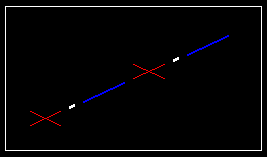
\includegraphics[width=\linewidth]{images/line.png}
\end{minipage}


\newpage
\hypertarget{box}{}
\subsubsection*{Box-Element}
The \texttt{Box}-Element is used to specify a box to be drawn in the UI.
\begin{center}
    \texttt{<box>} | \texttt{<b>}
\end{center}

\renewcommand{\arraystretch}{1.3}
\begin{tcolorbox}[colback=white, colframe=black!75, title=Arguments]
\begin{tabularx}{\linewidth}{p{60pt}|p{110pt}|X}
\textbf{Name} & \textbf{Values} & \textbf{Description}\\
\hline
colors/ color/ col & tag:color;... & Defines tag-based colors for rendering. Colors can be RGB tuples (r,g,b) or names (e.g., "red"). "inv" or "none" make elements invisible. If no tag is specified (e.g., "color=red"), the default tag '' is used. Default: inv\\
\rowcolor[HTML]{E8E8E8}
fillmode(s)/ fill(s)/ altmode(s)/ mode(s) & tag:mode;... & Sets the fill pattern for sub-boxes: striped vertically/horizontally or checkerboard. Values: striped\_vert (strv), striped\_hor (strh), checkerboard (cb). Uses default tag '' if none given. Default: solid\\
fillsize(s)/ innersizing(s)/ size(s) & tag:int|float;... & Sets size of the alternating pattern, either absolute or relative. Uses default tag '' if none given. Default: 10\\
\rowcolor[HTML]{E8E8E8}
inset & float|float,float| int|int,int & Sets padding inside the box. One value applies to both dimensions; two values specify width and height separately. Ints are absolute; floats are percentages. Default: 0\\
orders/ sectionorders/ ord & tag:tag1,tag2,...;... & Defines tag sequence used to render fill patterns cyclically in sub-boxes. Uses default tag '' if none given. Default: ''\\
\rowcolor[HTML]{E8E8E8}
partitioning/ part & intxint;[c1,c2,...]| [1=c1,3=c3,...]| 4=[...] & Splits the box into columns × rows of sub-boxes. Each sub-box can have its own fillmode, size, and filter defined by tags. Labels are set per row or column using square brackets. Sub-boxes have ''-tag per default. Default: 1x1\\
& EXPERIMENTAL & \\
\rowcolor[HTML]{E8E8E8}
filter(s)/ filt & tag:mode= float,float,float+float;... & Applies shape filters to sub-boxes. Modes: triangle/linear/quadratic/circle, with optional inversion ("i" prefix). Filters define a point and max distance for visible area. Default: nofilter
\end{tabularx}
\end{tcolorbox}

\begin{minipage}{0.35\linewidth}
Example (960×560):\\
    <box\\partitioning="4x2;[a,b,a,b][2=c,4=c]"\\filter="b:it=0.5,0.0,0.5+0.0"\\inset="80"\\colors=\\"(240,30,30);c1:(120,30,30);c2:(60,60,60)"\\fillmode="a:strh;b:cb;c:strv"\\fillsize="40"\\sectionorders=\\"c3;a:c1,c2;b:c1,c2;c:c1,c2"></box>
\end{minipage}
\hfill
\begin{minipage}{0.55\linewidth}
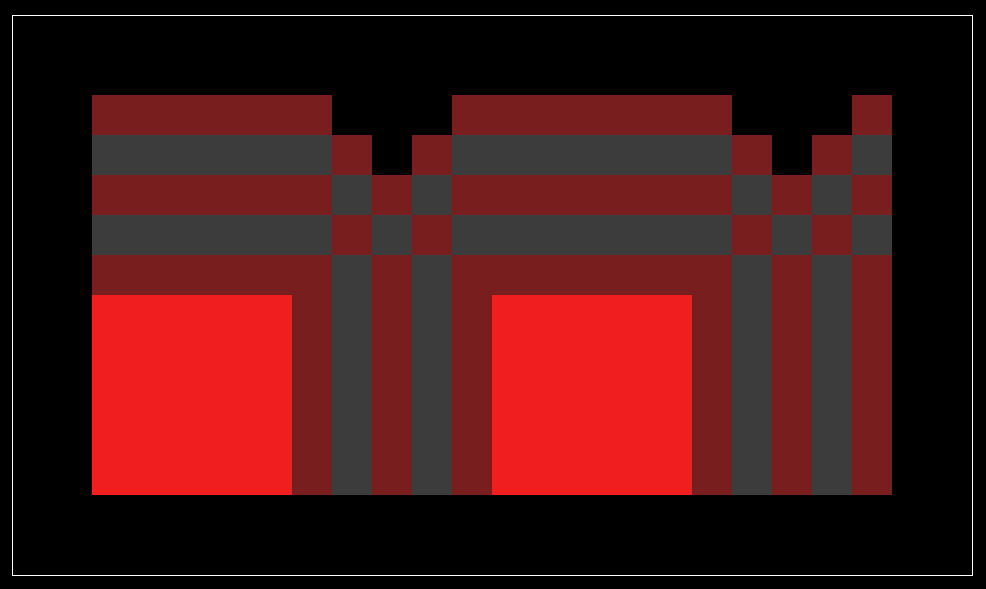
\includegraphics[width=\linewidth]{images/box.png}
\end{minipage}


\newpage
\hypertarget{text}{}
\subsubsection*{Text-Element}
The \texttt{Text}-Element is used to specify a text to be drawn in the UI.
\begin{center}
    \texttt{<text>} | \texttt{<t>}
\end{center}

\renewcommand{\arraystretch}{1.3}
\begin{tcolorbox}[colback=white, colframe=black!75, title=Arguments]
\begin{tabularx}{\linewidth}{p{50pt}|p{110pt}|X}
\textbf{Name} & \textbf{Values} & \textbf{Description}\\
\hline
align & float|l|r,float|t|b & Sets the align of the text inside the text-box. Default: 0.5,0.5\\
\rowcolor[HTML]{E8E8E8}
colors/ color/ col & color & Defines fontcolor for rendering. Color can be RGB tuple (r,g,b) or name (e.g., "red"). "inv" or "none" makes text invisible. Default: inv\\
fontname/ sysfont/ font & fontname;... & Sets font for rendering . Default: Arial\\
\rowcolor[HTML]{E8E8E8}
fontsize/ size & d|int|xxs|xs|...|xl|xxl;... & Sets fontsize for rendering. 'd' sets the fontsize to be dynamicly calculated. Default: 24\\
inset & float|float,float| int|int,int & Sets padding inside the box. One value applies to both dimensions; two values specify width and height separately. Ints are absolute; floats are percentages. Default: 0\\
\end{tabularx}
\end{tcolorbox}

\begin{minipage}{0.35\linewidth}
Example (640×360):\\
      <text\\inset="100"\\color="red"\\fontsize="l"\\align="0.3,0.9">\\Hello World\\</text>
\end{minipage}
\hfill
\begin{minipage}{0.55\linewidth}
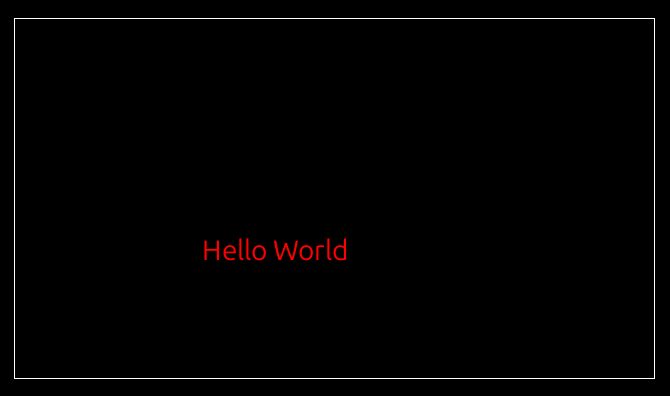
\includegraphics[width=\linewidth]{images/text.png}
\end{minipage}



\newpage
\hypertarget{framed}{}
\subsubsection*{Framed-Element}
The \texttt{Framed}-Element is used to wrap an element with an border and an background.
\begin{center}
    \texttt{<framed>} | \texttt{<fr> | \texttt{<f>}}
\end{center}

\renewcommand{\arraystretch}{1.3}
\begin{tcolorbox}[colback=white, colframe=black!75, title=Arguments]
\begin{tabularx}{\linewidth}{p{50pt}|p{110pt}|X}
\textbf{Name} & \textbf{Values} & \textbf{Description}\\
\hline
inset/ offset/ padding & int & Sets padding inside the box. Default: 0\\
\end{tabularx}
\end{tcolorbox}

\renewcommand{\arraystretch}{1.3}
\begin{tcolorbox}[colback=white, colframe=black!75, title=Children]
\begin{tabularx}{\linewidth}{p{50pt}|p{110pt}|X}
\textbf{Name} & \textbf{Amount} & \textbf{Description}\\
\hline
\hyperlink{line}{\texttt{Line}} & 0 - 4 & Sets the borders of the framed. If one is provided it is applied to all sides. If two are provided, the first is applied to left and right and the second to top and bottom. Otherwise borders are applied like 1-left, 2-right, 3-top, 4-bottom. Default: noborders\\
\rowcolor[HTML]{E8E8E8}
\hyperlink{box}{\texttt{Box}} & 0 - 1 & Sets the background of the framed. Default: nobackground\\
\texttt{Any Element} & 1 & Wrapped element.\\
\end{tabularx}
\end{tcolorbox}

Example (640×360):\\
<framed offset="50">\\
  <line color="inv;r:red" thickness="3" sizes="10;n:20" inset="0.1" sectionorder="r,n"></line>\\
  <line color="white"></line>\\
  <line color="inv;r:red" thickness="3" sizes="10;n:20" inset="0.1" sectionorder="r,n"></line>\\
  <box colors="(0,0,240);a:(0,120,0)" inset="0.05" fillmode="strv" sectionorders=",a" filter="c=0.5,0.5,0.5+0.5" fillsize="15"></box>\\
  <text inset="50" color="(160,120,160)" fontsize="d">Hello World</text>\\
</framed>
\begin{figure}[h]
    \centering
    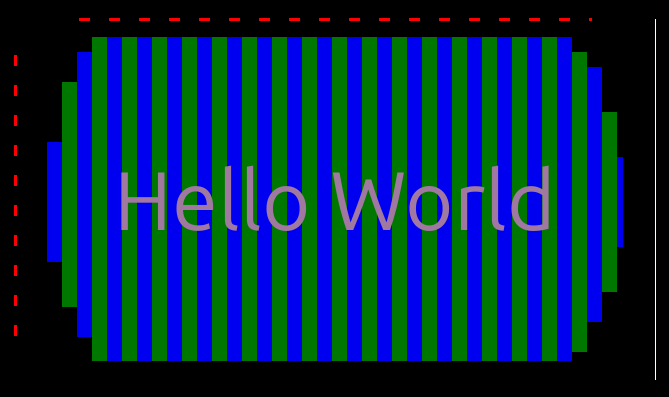
\includegraphics[width=0.5\linewidth]{images/framed.png}
\end{figure}



\newpage
\hypertarget{group}{}
\subsubsection*{Group-Element}
The \texttt{Group}-Element is used to group multiple elements together.
\begin{center}
    \texttt{<group>} | \texttt{<group>} | \texttt{<gr> | \texttt{<g>}}
\end{center}

\renewcommand{\arraystretch}{1.3}
\begin{tcolorbox}[colback=white, colframe=black!75, title=Arguments]
\begin{tabularx}{\linewidth}{p{50pt}|p{110pt}|X}
\textbf{Name} & \textbf{Values} & \textbf{Description}\\
\hline
horizontal/ hor & & Sets the group to align the elements horizontal. Default: vertical\\
\rowcolor[HTML]{E8E8E8}
offset/ spacing & int & Sets the spacing between elements in the group. Default: 0\\
size(s)/ sizing(s) & float|int=float,... & Sets the relative sizing of the elements inside the group. Default: 1.0\\
\end{tabularx}
\end{tcolorbox}

\renewcommand{\arraystretch}{1.3}
\begin{tcolorbox}[colback=white, colframe=black!75, title=Children]
\begin{tabularx}{\linewidth}{p{50pt}|p{110pt}|X}
\textbf{Name} & \textbf{Amount} & \textbf{Description}\\
\hline
\texttt{Any Element} & 1+ & Grouped elements.\\
\end{tabularx}
\end{tcolorbox}

Example (640×360):\\
<group spacing="40" hor="" sizings="0.5,0.3,0.2">\\
<group spacing="20" sizing="2=1.4">\\
<box color="red"></box>\\
<box color="(160,0,0)"></box>\\
<box color="(80,0,0)"></box>\\
</group>\\
<box color="green"></box>\\
<box color="blue"></box>\\
</group>

\begin{figure}[h]
    \centering
    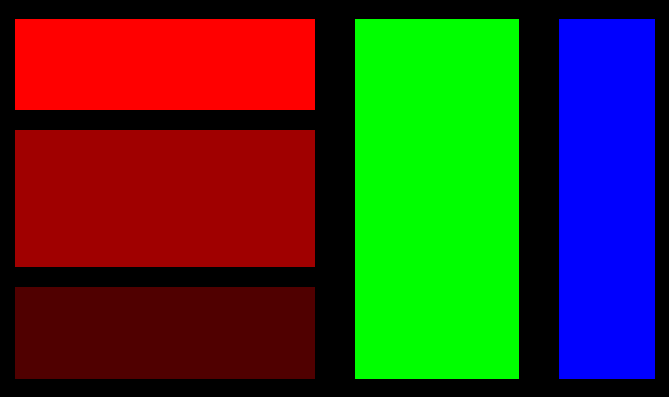
\includegraphics[width=0.5\linewidth]{images/group.png}
\end{figure}



\newpage
\hypertarget{dropdown}{}
\subsubsection*{Dropdown-Element}
The \texttt{Dropdown}-Element is used to create a dropdown.
\begin{center}
    \texttt{<dropdown>} | \texttt{<dpd>}
\end{center}

\renewcommand{\arraystretch}{1.3}
\begin{tcolorbox}[colback=white, colframe=black!75, title=Arguments]
\begin{tabularx}{\linewidth}{p{50pt}|p{110pt}|X}
\textbf{Name} & \textbf{Values} & \textbf{Description}\\
\hline
horizontal/ hor & & Sets the dropdown to be horizontal. Default: vertical\\
\rowcolor[HTML]{E8E8E8}
offset/ spacing & int & Sets the spacing between elements in the dropdown. Default: 0\\
size(s)/ sizing(s) & float|int=float,... & Sets the relative sizing of the elements inside the dropdown. Default: 1.0\\
\end{tabularx}
\end{tcolorbox}

\renewcommand{\arraystretch}{1.3}
\begin{tcolorbox}[colback=white, colframe=black!75, title=Children]
\begin{tabularx}{\linewidth}{p{50pt}|p{110pt}|X}
\textbf{Name} & \textbf{Amount} & \textbf{Description}\\
\hline
\texttt{Any Element} & 1+ & First element is the one to click to reveal the other elements as dropdown.\\
\end{tabularx}
\end{tcolorbox}

Example (128×72):\\
<dpd spacing="10" hor="" sizings="0.5,0.3,0.2,c5=1.2">\\
<box color="green"></box>\\
<dpd spacing="20" sizing="c2=1.9">\\
<box color="red"></box>\\
<box color="(160,0,0)"></box>\\
<box color="(80,0,0)"></box>\\
</dpd>\\
<box color="blue"></box>\\
<box color="green"></box>\\
<box color="blue"></box>\\
<box color="green"></box>\\
</dpd>

\begin{figure}[h]
    \centering
    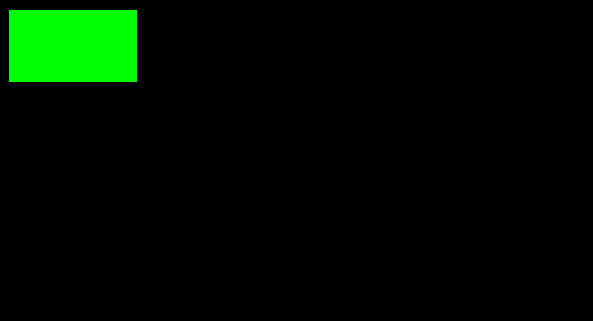
\includegraphics[width=0.45\linewidth]{images/dropdown1.png}
    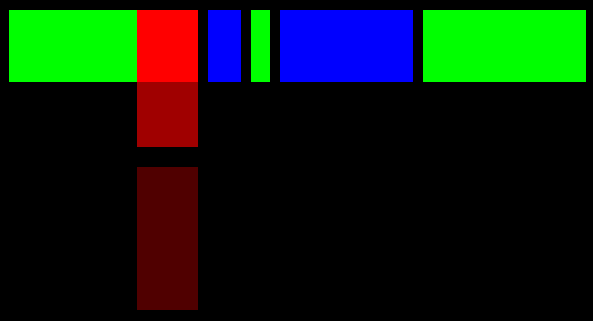
\includegraphics[width=0.45\linewidth]{images/dropdown2.png}
\end{figure}

\end{document}
